\documentclass[../../main.tex]{subfiles}
\begin{document}

\begin{flushright}
  \footnotesize\textit{【自動文字起こし・要確認】}
\end{flushright}

% Source: handwritten.pdf 第5問．
{\bf [解]}
$H$の方程式は$z=y-1$である．
$y=2\sin\theta$ $(\dfrac{\pi}{6}\leqq\theta\leqq\dfrac{\pi}{2})$で切断する切り口は下図で，
この面積$S(\theta)$として
\begin{align}S(\theta)=4\cos\theta(2\sin\theta-1).
\end{align}
\begin{figure}[H]
  \centering
  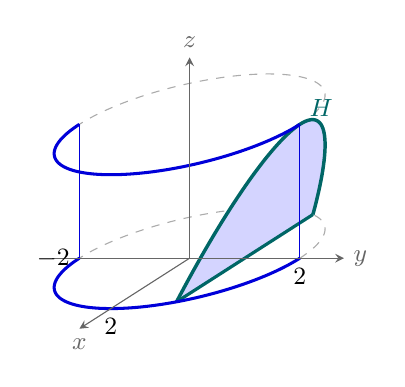
\begin{tikzpicture}[x={(-.5cm,-.32cm)},y={(.7cm,0cm)},z={(0cm,1.7cm)},
    >=stealth,every node/.style={font=\small}]
    % 円柱の奥側と手前側の輪郭を描き分ける。
    \draw[dashed,gray!65,domain=90:270,samples=70]
    plot ({2*cos(\x)},{2*sin(\x)},0);
    \draw[dashed,gray!65,domain=90:270,samples=70]
    plot ({2*cos(\x)},{2*sin(\x)},1);
    \fill[blue!17] plot[domain=30:150,samples=70]
    ({2*cos(\x)},{2*sin(\x)},{2*sin(\x)-1}) -- cycle;
    \draw[teal!80!black,line width=1.25pt,domain=30:150,samples=70]
    plot ({2*cos(\x)},{2*sin(\x)},{2*sin(\x)-1});
    \draw[teal!80!black,line width=1.15pt]
    ({sqrt(3)},1,0)--({-sqrt(3)},1,0);
    \draw[blue!85!black,line width=1.1pt,domain=-90:90,samples=70]
    plot ({2*cos(\x)},{2*sin(\x)},0);
    \draw[blue!85!black,line width=1.1pt,domain=-90:90,samples=70]
    plot ({2*cos(\x)},{2*sin(\x)},1);
    \draw[blue!85!black] (0,-2,0)--(0,-2,1) (0,2,0)--(0,2,1);
    \draw[->,gray!80!black] (0,0,0)--(2.8,0,0) node[below] {$x$};
    \draw[->,gray!80!black] (0,-2.5,0)--(0,2.8,0) node[right] {$y$};
    \draw[->,gray!80!black] (0,0,0)--(0,0,1.5) node[above] {$z$};
    \node[right,teal!80!black] at (0,2,1.12) {$H$};
    \node[below] at (0,2,0) {$2$};
    \node[left] at (0,-2,0) {$-2$};
    \node[below] at (2,0,0) {$2$};
  \end{tikzpicture}
  \qquad
  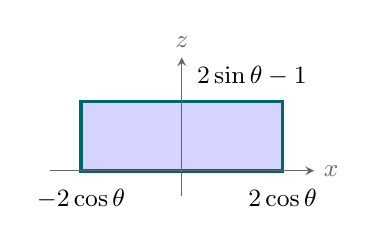
\begin{tikzpicture}[x=.8cm,y=.8cm,>=stealth,
    every node/.style={font=\small}]
    \fill[blue!17] (-1.6,0) rectangle (1.6,1.1);
    \draw[teal!80!black,line width=1.25pt] (-1.6,0) rectangle (1.6,1.1);
    \draw[->,gray!80!black] (-2.1,0)--(2.1,0) node[right] {$x$};
    \draw[->,gray!80!black] (0,-.4)--(0,1.8) node[above] {$z$};
    \node[below=3pt] at (-1.6,0) {$-2\cos\theta$};
    \node[below=3pt] at (1.6,0) {$2\cos\theta$};
    \node[above right=2pt] at (0,1.1) {$2\sin\theta-1$};
  \end{tikzpicture}
  \caption{円柱を平面$H$で分けた部分と$y=2\sin\theta$での切り口}
\end{figure}
だから，以下$c=\cos\theta$，$s=\sin\theta$として，求める体積$V$は
\begin{align}
  \begin{split}
    V&=\int_1^2S(\theta)\,d(2s)\\
    &=\int_{\pi/6}^{\pi/2}S(\theta)\dfrac{d(2s)}{d\theta}\,d\theta\\
    &=\int_{\pi/6}^{\pi/2}4c(2s-1)\,2c\,d\theta\\
    &=8\int_{\pi/6}^{\pi/2}(2c^2s-c^2)\,d\theta\\
    &=8\left[-\dfrac{2}{3}c^3\right]_{\pi/6}^{\pi/2}
    -8\cdot\dfrac{1}{2}\left[\theta+\dfrac{1}{2}\sin2\theta\right]_{\pi/6}^{\pi/2}\\
    &=\dfrac{16}{3}\left(\dfrac{\sqrt{3}}{2}\right)^3
    -4\left(\dfrac{\pi}{3}-\dfrac{1}{2}\cdot\dfrac{\sqrt{3}}{2}\right)\\
    &=3\sqrt{3}-\dfrac{4}{3}\pi.
  \end{split}
\end{align}

\end{document}
